\subsection{Multiplicity dependence of hard probes}

\subsubsection{Sequential melting of quarkonia states}

Effects affecting sequentially the $\Upsilon$ excited states with the increase 
of the overall event activity (or multiplicity) are observed in pPb collisions 
at \roots\ = 5.02 TeV by CMS~\cite{Chatrchyan:2013nza}. Up to these measurements, 
such a phenomenon was almost exclusively considered only in context of the formation 
of a quark-gluon plasma in ultrarelativistic central AA collisions, 
where it is considered as one of the golden signatures of the creation of 
such a deconfined QCD medium. Therefore, it is of great interest to directly
compare the sequential suppression effects of $\Upsilon$ states in small (pPb) and
large (PbPb) systems as a function of multiplicity.

Because of limited available data in 2013 run, the pPb data of 
$[\Upsilon(2S) / \Upsilon(1S)]$ ratio were only explored over a multiplicity 
regime right below the range covered by the measurements in PbPb collisions.
This prevents a conclusive answer on whether or not there is a continuous decrease
in the $[\Upsilon(2S) / \Upsilon(1S)]$ ratio going from pPb to PbPb systems.
A significantly larger pPb data sample at \rootsNN\ = 8.16 TeV 
in 2016 will bridge the gap existing now between pPb and PbPb data, which 
helps to make a quantitative statement about the phenomena affecting 
quarkonium production from small (pp, pPb) to large (PbPb), high-density QCD environments. 


\begin{figure}[thb]
  \begin{center}
    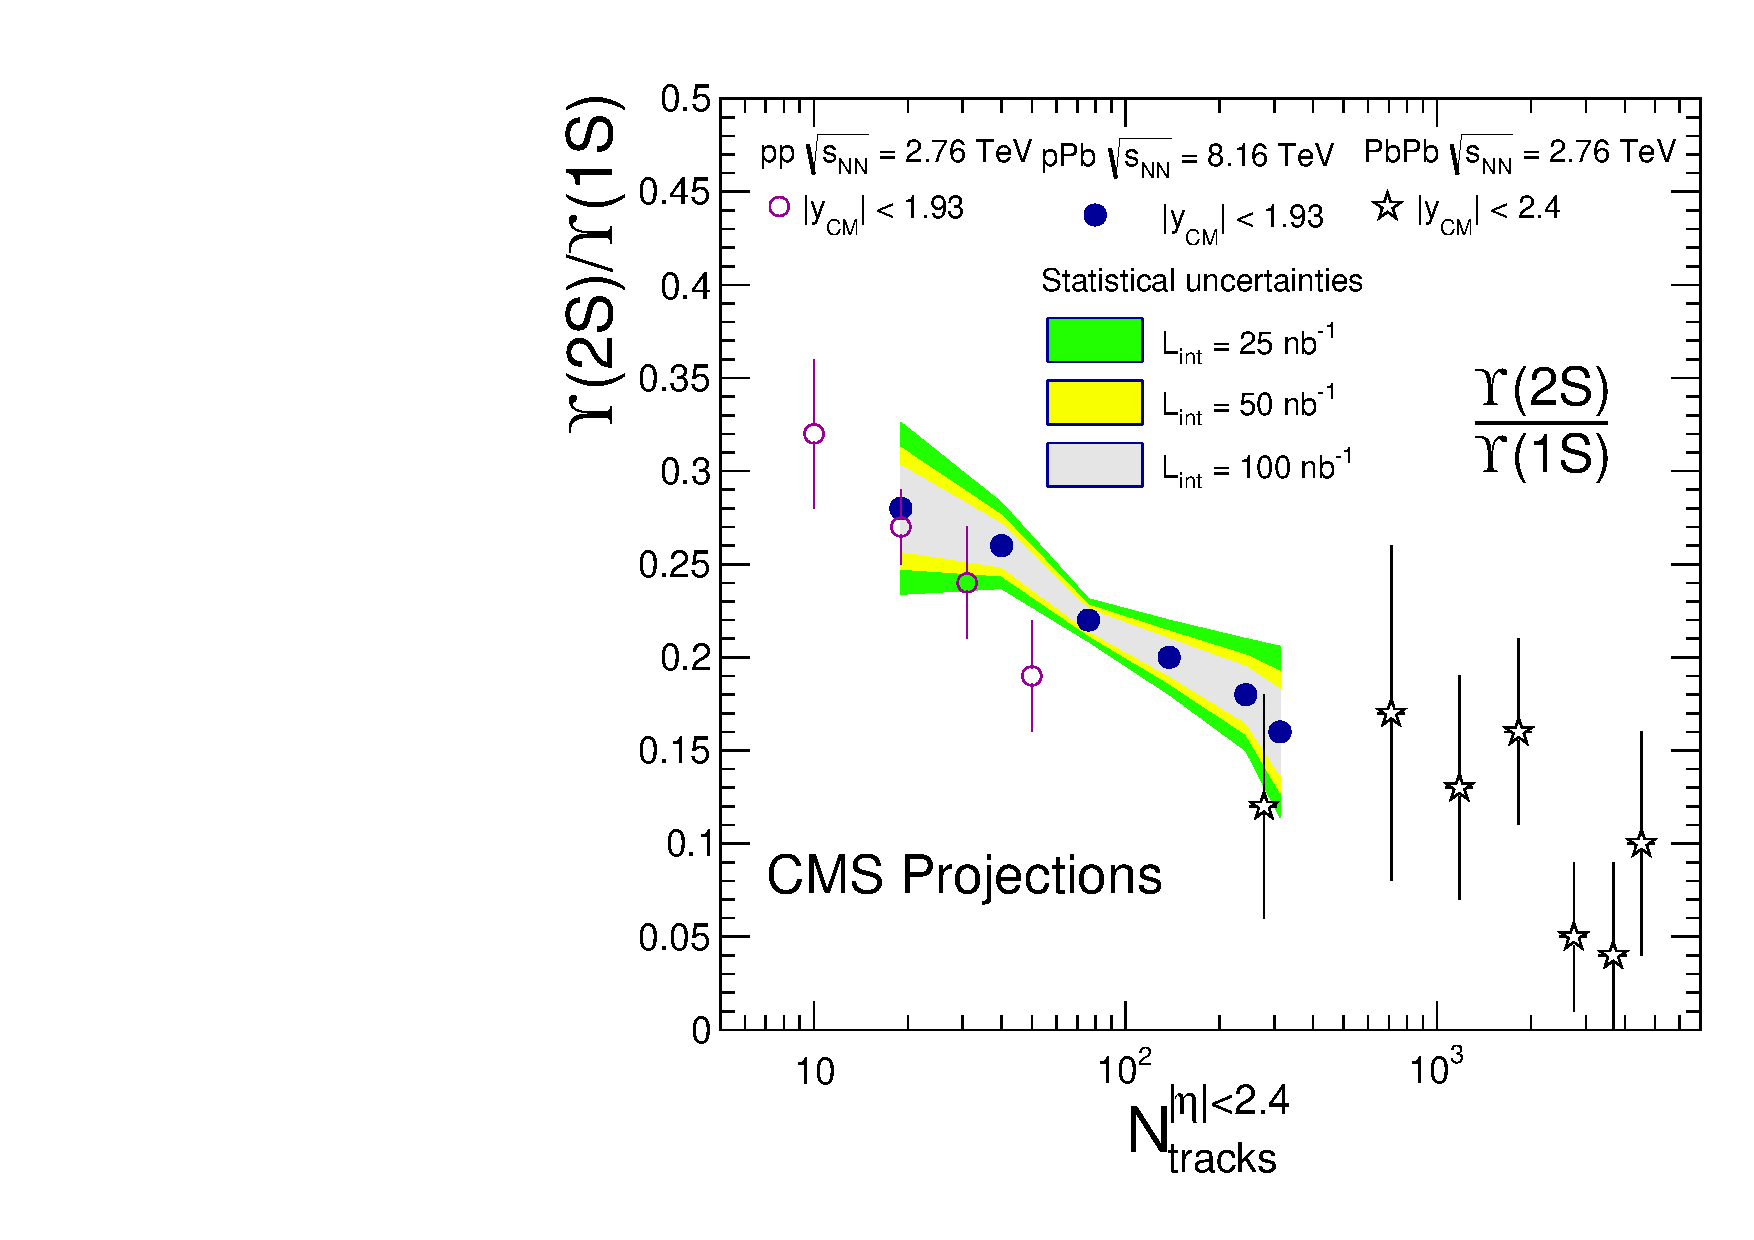
\includegraphics[width=0.6\textwidth]{figures/Upsilon_pPb_proj_combineLumi.pdf}
    \caption{ The single ratios $[\Upsilon(2S) / \Upsilon(1S)]$ for $|y_{CM}|<1.93$ 
    as a function of charged-particle multiplicity, projected to be measured in pPb collisions 
    \rootsNN\ = 8.16 TeV (closed circles) for three luminosity scenarios of L$_{\rm int}$ = 
    25, 50 and 100 nb$^{-1}$. The pp (open circles) and PbPb (stars) (measured in $|y_{CM}|<2.4$) 
    ratios at $\roots = 2.76$ TeV are added for comparison.
    }
    \label{fig:UpsilonvsNtrk}
  \end{center}
\end{figure} 

In Fig.~\ref{fig:UpsilonvsNtrk}, the projected statistical uncertainties 
of the $[\Upsilon(2S) / \Upsilon(1S)]$ ratio measurement for $|y_{CM}|<1.93$ as a 
function of charged-particle multiplicity is presented, assuming three different 
luminosity scenarios of L$_{\rm int}$ = 100, 50 and 25 nb$^{-1}$ for the 8.16 TeV pPb run in 2016. 
The projections are obtained by considering the raw yields measured in the 2013 pPb 
sample used in Ref.~\cite{Chatrchyan:2013nza} and scaling the statistical uncertainties 
based on the projected multiplicity distribution in Fig.~\ref{fig:Ntrk_pPb} under
different luminosity scenario. Note that the uncertainties of PbPb data are also expected to
reduce significantly with run-2 data in 2015 and 2018. With an integrated luminosity of 
100 nb$^{-1}$ pPb collisions at \rootsNN\ = 8.16 TeV, the pPb and PbPb data
will be compared with high precision over a common multiplicity range.


\subsection{Azimuthal anisotropy of Charmonia from pPb to PbPb}


\begin{figure}[thb]
  \begin{center}
    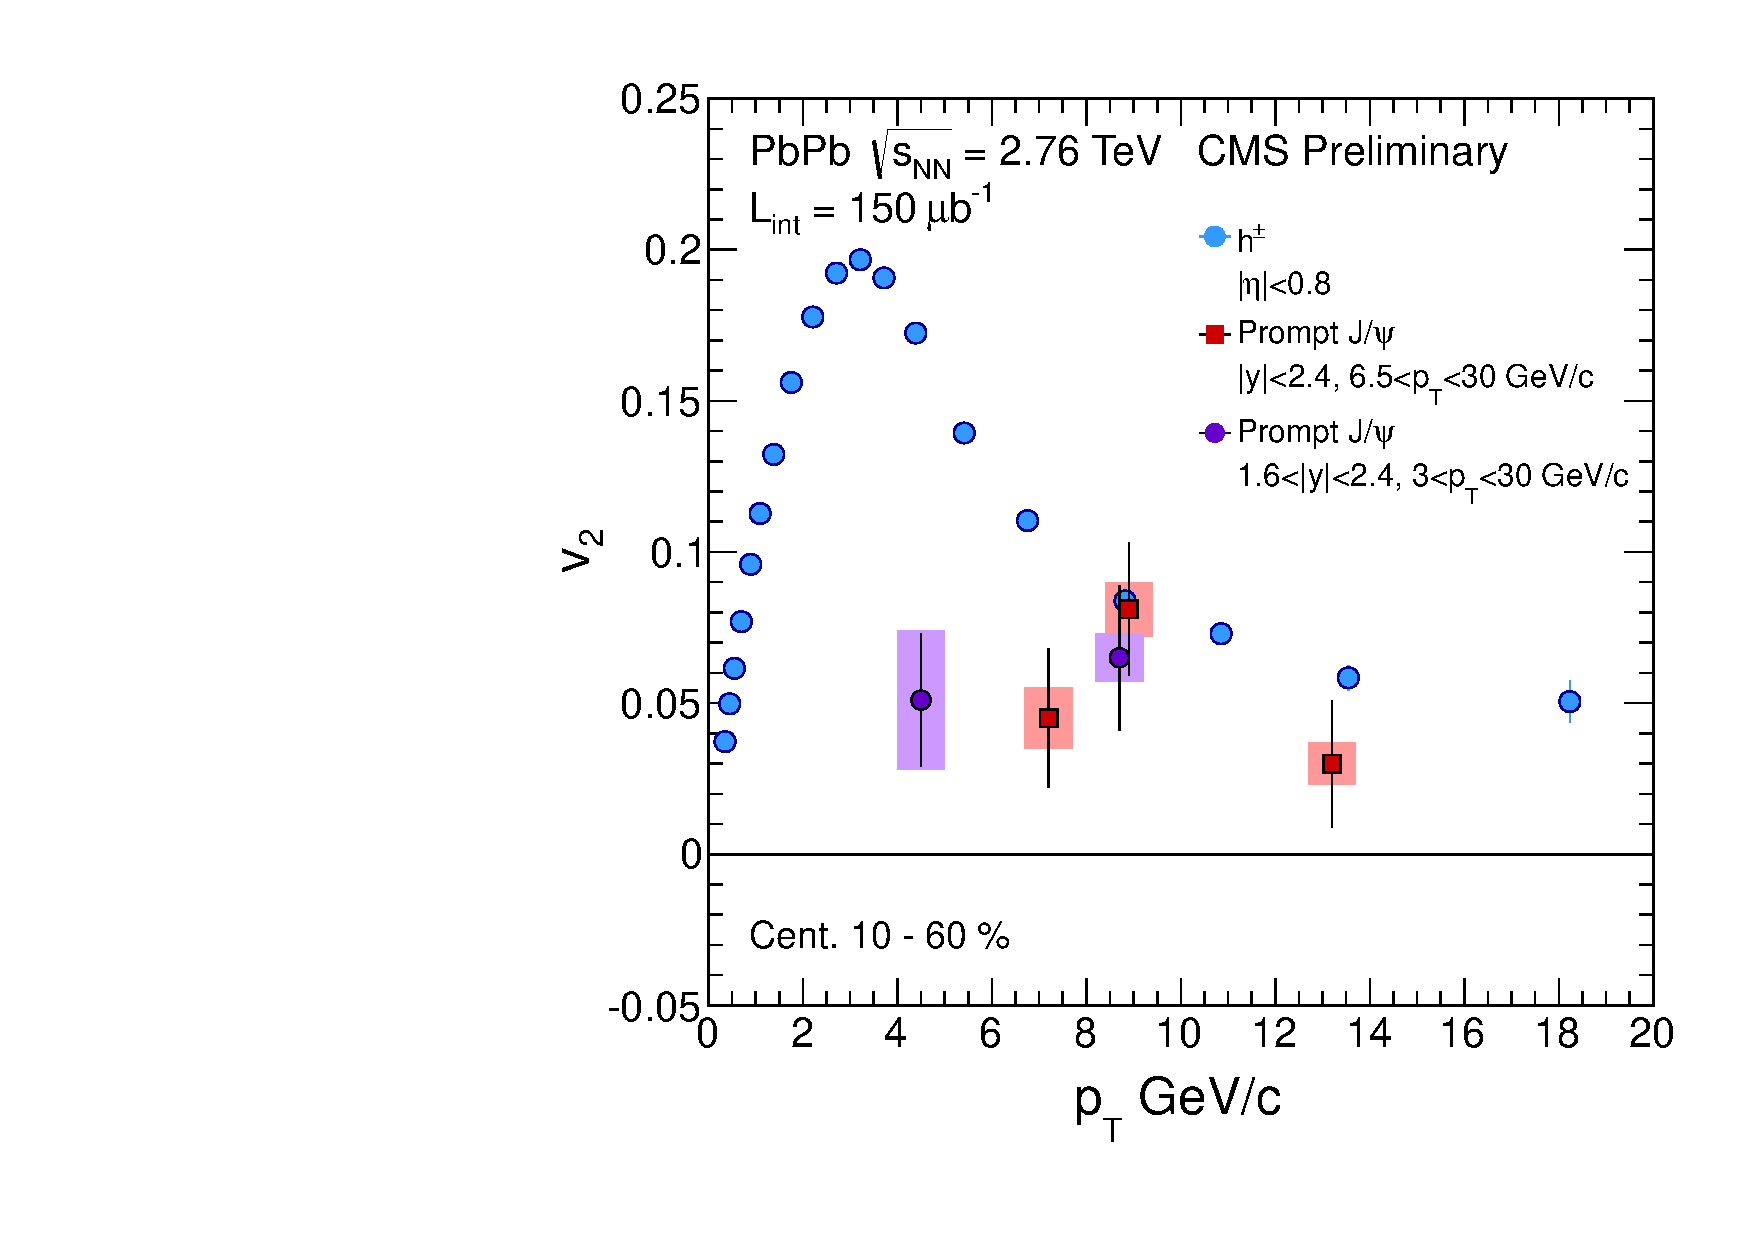
\includegraphics[width=0.6\textwidth]{figures/comp_v2_pTs_CMSflow_Prp_Cor.pdf}
    \caption{ The $v_2$ values of prompt $J/\Psi$ as a function of \pt, compared to the 
    charged hadron data in the same event centrality class of 10-60\% at $\rootsNN = 2.76$ TeV,
    measured by CMS.}
    \label{fig:v2_Jpsi}
  \end{center}
\end{figure} 

Viewed as one of the golden probes of the QGP formation in heavy-ion collisions, it is highly
interesting to broaden the scope of measurements on quarkonia states in high-multiplicity pPb
collisions to seek for hints of QGP formation there. In light of similar 
collective anisotropy effects measured for light hadrons in pPb and PbPb collisions, 
a measurement of $J/\Psi$ $v_2$ in high-multiplicity pPb collisions may provide an 
indication of the existence of a medium, in which the charm quarks flow and then 
recombine into $J/\Psi$ states. 

The $v_2$ of prompt $J/\Psi$ in PbPb collisions at \rootsNN\ = 2.76 TeV has been measured by CMS
as a function of \pt\ in 10--60\% centrality class~\cite{CMS-PAS-HIN-12-001}. Within uncertainties,
positive values of prompt $J/\Psi$ $v_2$ are found to be significant and seem to follow the same trend
as the light charged particles. Such a measurement in high-multiplicity pPb collisions will be highly interesting as it may provide an indication of the existence of a medium, in which the charm quarks flow and
recombine into $J/\Psi$ particles. 

To estimate the feasibility of such a measurement in 2016 pPb run at \rootsNN\ = 8.16 TeV, 
there are about 12,000 $J/\Psi$ signals used in the PbPb results presented in Fig.~\ref{fig:v2_Jpsi}.
From 2013 pPb run with an integrated luminosity of 35 nb$^{-1}$, approximately 21,000 $J/\Psi$ signals
are recorded for top 10\% highest-multiplicity pPb events. With an integrated luminosity of 100 nb$^{-1}$
pPb data at \rootsNN\ = 8.16 TeV in 2016, a factor of 4 increase in the data sample 
for this multiplicity range is expected, projecting to a total of about 84, 000 $J/\Psi$ signals, which
makes a measurement of $J/\Psi$ $v_2$ promising.